\begin{frame}[fragile]

  {\Huge Graph Kernels}

  \vspace{10pt}

  {\large Kokkos Kernels functionality for graph computations.}

  \vspace{20pt}

  \textbf{Learning objectives:}
  \begin{itemize}
    \item {Distance-1 Graph Coloring}
    \item {Distance-2 Graph Coloring}
    \item {Bipartite Graph Partial Coloring}
  \end{itemize}

  \vspace{-20pt}

\end{frame}

%==========================================================================

\begin{frame}[fragile]{Distance-1 Coloring}

\textbf{Distance-1 Graph Coloring}

\begin{itemize}
  \item Given a graph, assign a color to each vertex so that no two adjacent vertices have the same color
  \item Minimizing the number of unique colors is NP-hard
  \item Approximate solution (with a few more colors than optimal) is still useful
  \item KokkosKernels has two main algorithms for this: vertex-based and edge-based
\end{itemize}
\end{frame}

\begin{frame}[fragile]{Distance-1 Graph Coloring}
\textbf{Vertex-Based (VB) Coloring}

Initialize worklist containing every vertex.
\begin{itemize}
  \item In parallel, for each vertex v in worklist:
  \begin{itemize}
    \item Assign smallest color to v which isn't found on any neighbor
  \end{itemize}
  \item In parallel, for each vertex v in worklist:
  \begin{itemize}
    \item If v's color is matches with a neighbor, uncolor v and add it to next worklist
  \end{itemize}
\end{itemize}
These steps are repeated until the worklist is empty (all vertices have been colored).
\end{frame}

\begin{frame}[fragile]{Distance-1 Graph Coloring}
\textbf{Edge-Based (EB) Coloring}

Initialize worklist containing every edge.
\begin{itemize}
  \item In parallel, for each edge e in worklist:
  \begin{itemize}
    \item If both endpoints of e have the same color, uncolor the one with a higher ID
    \item If at least one endpoint of e is uncolored, add e to the next worklist.
  \end{itemize}
  \item In parallel, for each edge e in worklist:
  \begin{itemize}
    \item If exactly one endpoint is colored, add that color to forbidden set for other endpoint
  \end{itemize}
  \item In parallel, for each uncolored vertex v:
  \begin{itemize}
    \item Color v with smallest non-forbidden color
  \end{itemize}
\end{itemize}
These steps are repeated until the edge worklist is empty, meaning both endpoints of every edge have been colored.
\end{frame}

\begin{frame}[fragile]{Distance-1 Graph Coloring}
\textbf{Algorithm Summary}

\begin{itemize}
  \item EB pseudocode was simplified, did not include tentative coloring (technique for faster convergence)
  \item In VB, work per thread requires loop over neighbors of a vertex
  \item In EB, work per thread is constant time, but the worklists are longer
  \item EB is significantly faster on GPUs when the maximum degree is high (generally, $> 3000$)
  \item Otherwise, VBBIT (VB with bitwise operations to track forbidden colors) is usually the fastest.
  \item Use enum values \verb!KokkosGraph::COLORING_VBBIT! and \verb!KokkosGraph::COLORING_EB! 
\end{itemize}
\end{frame}

\begin{frame}[fragile]{Distance-1 Graph Coloring}
\textbf{Using Distance-1 Coloring}

\begin{code}
  #include "KokkosGraph_Distance1Color.hpp"
  KokkosKernels::KokkosKernelsHandle<...> handle;
  // Choose algorithm and set up
  handle.create_graph_coloring_handle(KokkosGraph::COLORING_VB);
  // Compute the coloring
  KokkosGraph::Experimental::graph_color(&handle,
    numVertices, numVertices, rowmap, entries);
  // Get the subhandle for coloring
  auto colorHandle = handle.get_graph_coloring_handle();
  // Get the number of colors used, and color labels
  auto numColors = colorHandle->get_num_colors();
  auto colors = colorHandle->get_vertex_colors();
  // Clean up
  handle.destroy_graph_coloring_handle();
\end{code}
\end{frame}

\begin{frame}[fragile]{Distance-2 Coloring and BGPC}
\textbf{Distance-2 Coloring Problem}

\begin{itemize}
  \item Each vertex must have a different color than all vertices within 2 hops of it
  \item If $G$ is represented by adjacency matrix, this is equivalent to computing distance-1 coloring on $G^2$
  \item Graph must be undirected (symmetric adjacency matrix)
\end{itemize}
\end{frame}

\begin{frame}[fragile]{Distance-2 Coloring and BGPC}
\textbf{Distance-2 Coloring Problem}

In this graph, 0 couldn't have the same color as 1 or 2, but it could have the same as 3 or 4.
\begin{figure}[h]
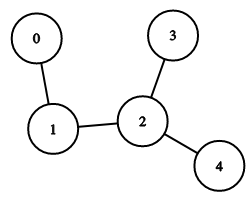
\includegraphics[width=0.5\textwidth]{figures/dist2_graph_example}
\end{figure}
\end{frame}

\begin{frame}[fragile]{Distance-2 Coloring and BGPC}
\textbf{Bipartite Graph Partial Coloring}

\begin{itemize}
  \item Closely related to distance-2 coloring
  \item Color either left or right side of a bipartite graph so that any vertices 2 hops apart have different colors
  \item Left-side BGPC equivalent to distance-1 coloring on $GG^\top$
  \item Right-side BGPC equivalent to distance-1 coloring on $G^{\top}G$
\end{itemize}
\end{frame}

\begin{frame}[fragile]{Distance-2 Coloring and BGPC}
\textbf{Bipartite Graph Partial Coloring}
\begin{itemize}
  \item For left-sided coloring of this graph, 1 couldn't have the same color as 0, but could have the same as 2.
  \item For right-sided coloring of this graph, vertices 3, 4 and 5 must all have different colors.
\end{itemize}
\begin{figure}[h]
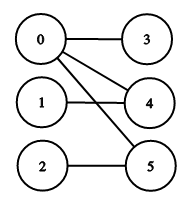
\includegraphics[width=0.4\textwidth]{figures/bgpc_example}
\end{figure}
\end{frame}

\begin{frame}[fragile]{Distance-2 Coloring and BGPC}
\textbf{D2/BGPC Algorithms}
\begin{itemize}
  \item VB (\verb!KokkosGraph::COLORING_D2_VB_BIT!): Just like distance-1 VB, but coloring and conflict resolution loop over neighbors-of-neighbors, not just neighbors
  \item NB (\verb!KokkosGraph::COLORING_D2_NB_BIT!) Net-based coloring from ``Greed is Good: Parallel Algorithms for BGPC'' by Ta\c{s} et al.
    Is asymptotically faster than VB by avoiding neighbors-of-neighbors loops, and is faster in practice.
\end{itemize}
\end{frame}

\begin{frame}[fragile]{Distance-2 Coloring and BGPC}
\textbf{Using Distance-2 Coloring}

\begin{code}
  #include "KokkosGraph_Distance2Color.hpp"
  KokkosKernels::KokkosKernelsHandle<...> handle;
  // Set up for coloring, and choose algorithm
  handle.create_distance2_graph_coloring_handle(
    KokkosGraph::COLORING_D2_NB_BIT);
  // Compute the coloring
  KokkosGraph::Experimental::graph_color_distance2(
    &handle, numVertices, rowmap, entries);
  // Get the subhandle for D2 coloring
  auto colorHandle =
    handle.get_distance2_graph_coloring_handle();
  auto numColors = colorHandle->get_num_colors();
  auto colors = colorHandle->get_vertex_colors();
  handle.destroy_distance2_graph_coloring_handle();
\end{code}
\end{frame}

\begin{frame}[fragile]{Distance-2 Coloring and BGPC}
\textbf{Using BGPC} 

Same handle and algorithm choices as D2, but use:
\begin{code}
KokkosGraph::Experimental::bipartite_color_rows(
  &handle, numRows, numColumns, rowmap, entries);
\end{code}

and:

\begin{code}
KokkosGraph::Experimental::bipartite_color_columns(
  &handle, numRows, numColumns, rowmap, entries);
\end{code}
\end{frame}

\begin{frame}[fragile]{Exercise}
\textbf{Coloring Exercise}
\begin{itemize}
  \item \verb!Intro-Full/Exercises/kokkoskernels/GraphColoring!
  \item Compute both D1 and D2 colorings of a graph
  \item The graph is generated as a 9-point stencil on a small 2D grid
  \item The colors will be printed out in the layout of the grid
\end{itemize}
\begin{figure}[h!]
  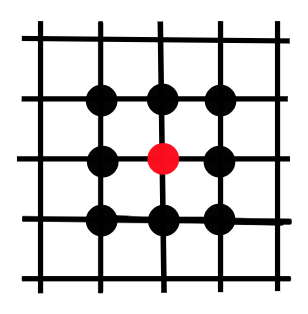
\includegraphics[width=0.3\textwidth]{figures/9pt_stencil.png}
  \caption{A 9-point stencil. The black points are adjacent to the red point.}
\end{figure}

\end{frame}

\begin{frame}[fragile]{Summary}
\textbf{Summary: Graph Algorithms}
\begin{itemize}
  \item Distance-1 Coloring
  \begin{itemize}
    \item vertex-based (VB) and edge-based (EB) based algorithms
    \item Use \verb!COLORING_VBBIT!, unless maximum degree $> 3000$ - then use \verb!COLORING_EB!
  \end{itemize}
  \item Distance-2 and Bipartite Graph Partial Coloring
  \begin{itemize}
    \item vertex-based (VB) and net-based (NB) algorithms
    \item Use \verb!COLORING_D2_NB_BIT! for best performance
  \end{itemize}
\end{itemize}

\end{frame}
